\chapter{具体需求}
\iffalse
<The following sections must be repeated for each requirement. >

在每一条需求描述中重复下列部分
\fi
\section{功能需求}
\iffalse
This section describes how the input of the software is translated to the output. It describes the essential action the software must perform.

For each kind of function, or each independent function in some cases, the requirements of input, process and output must be described, which are usually organized with the following four subsections:

本子章节应描述软件产品的输入怎样被转换成输出。它描述了软件必须执行的基本动作。 

对每一类功能或有时对每一个单独的功能,必须描述输入、处理、输出方面的需求。这些通常以下面四个子段落来组织:
\fi
\subsection{Android客户端功能需求}
\subsubsection{简介}
随着Android平台日益普及,的Android客户端是该即时通讯产品的主要客户端,拥有该产品的所有完整功能。
\begin{itemize}
\item 通讯模式
  \begin{itemize}  	
  	\item 用户一对一通讯
  	\item 群聊
  	\item 随机匹配聊天
  \end{itemize}
\item 通讯方式
  \begin{itemize}
  	\item 文字即时通讯
  	\item 图片、视频、音频、链接、文件等多种媒体的发送
  	\item 语音、视频及时通讯
  	\item 加密文字及时通讯
  \end{itemize}
\item 用户控制
  \begin{itemize}
  	\item 注册/注销账号
  	\item 添加/删除联系人
  	\item 加入/退出/创建群聊
  \end{itemize}
\end{itemize}
  \begin{figure}[!h]
	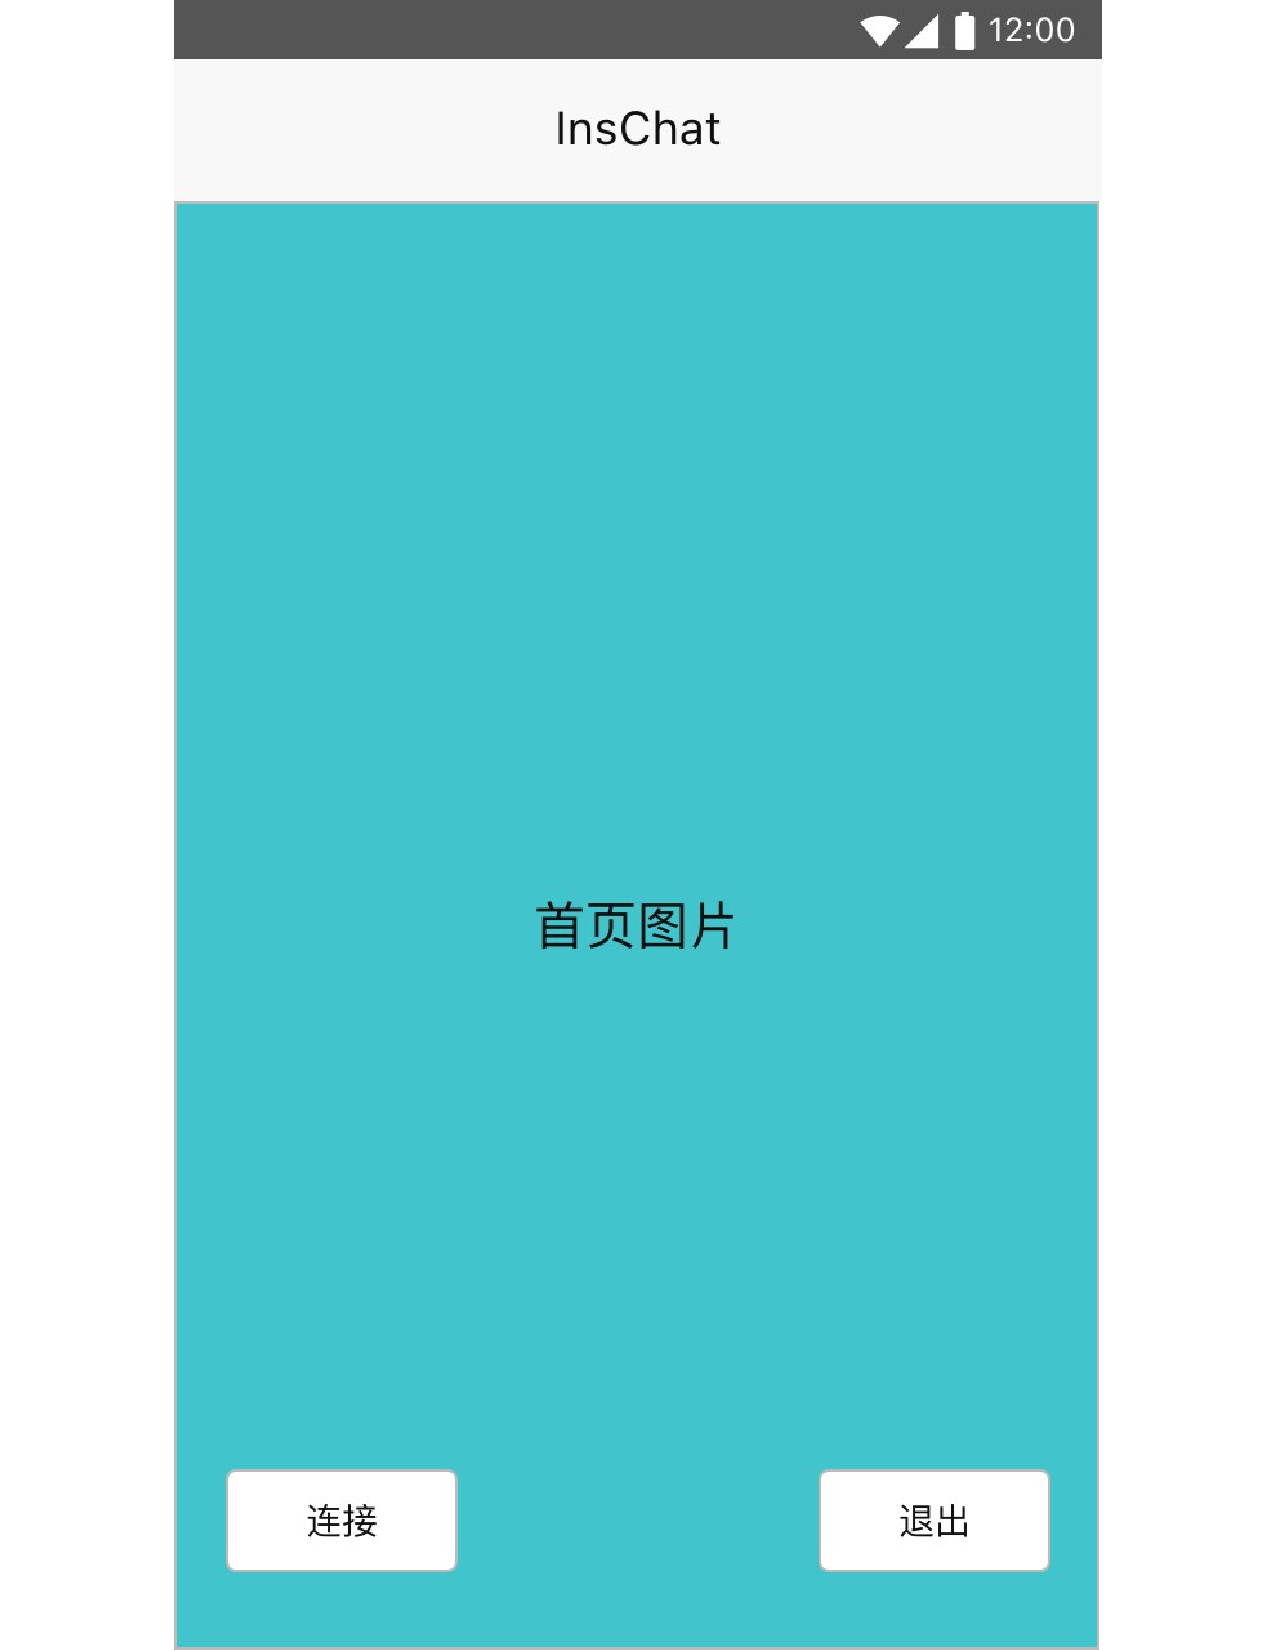
\includegraphics[width=8cm]{Page0}
	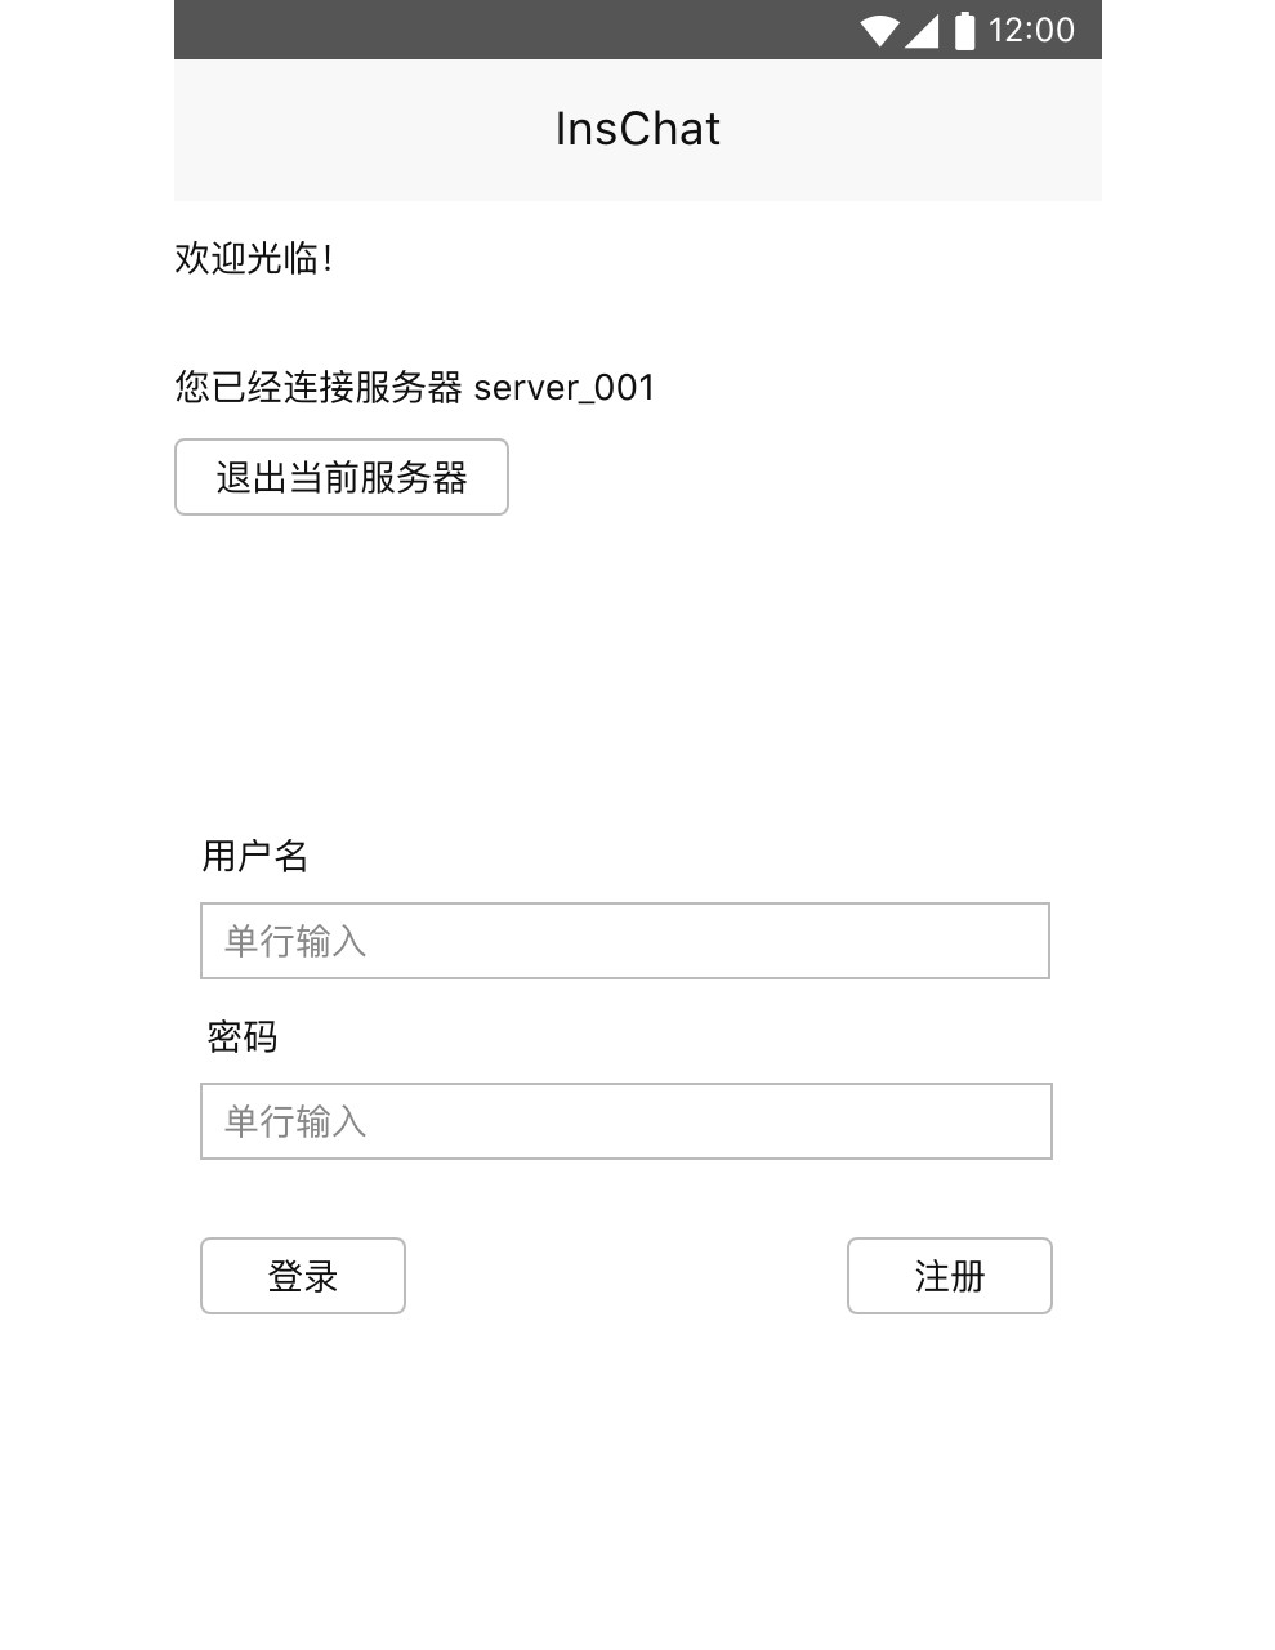
\includegraphics[width=8cm]{Page1}
	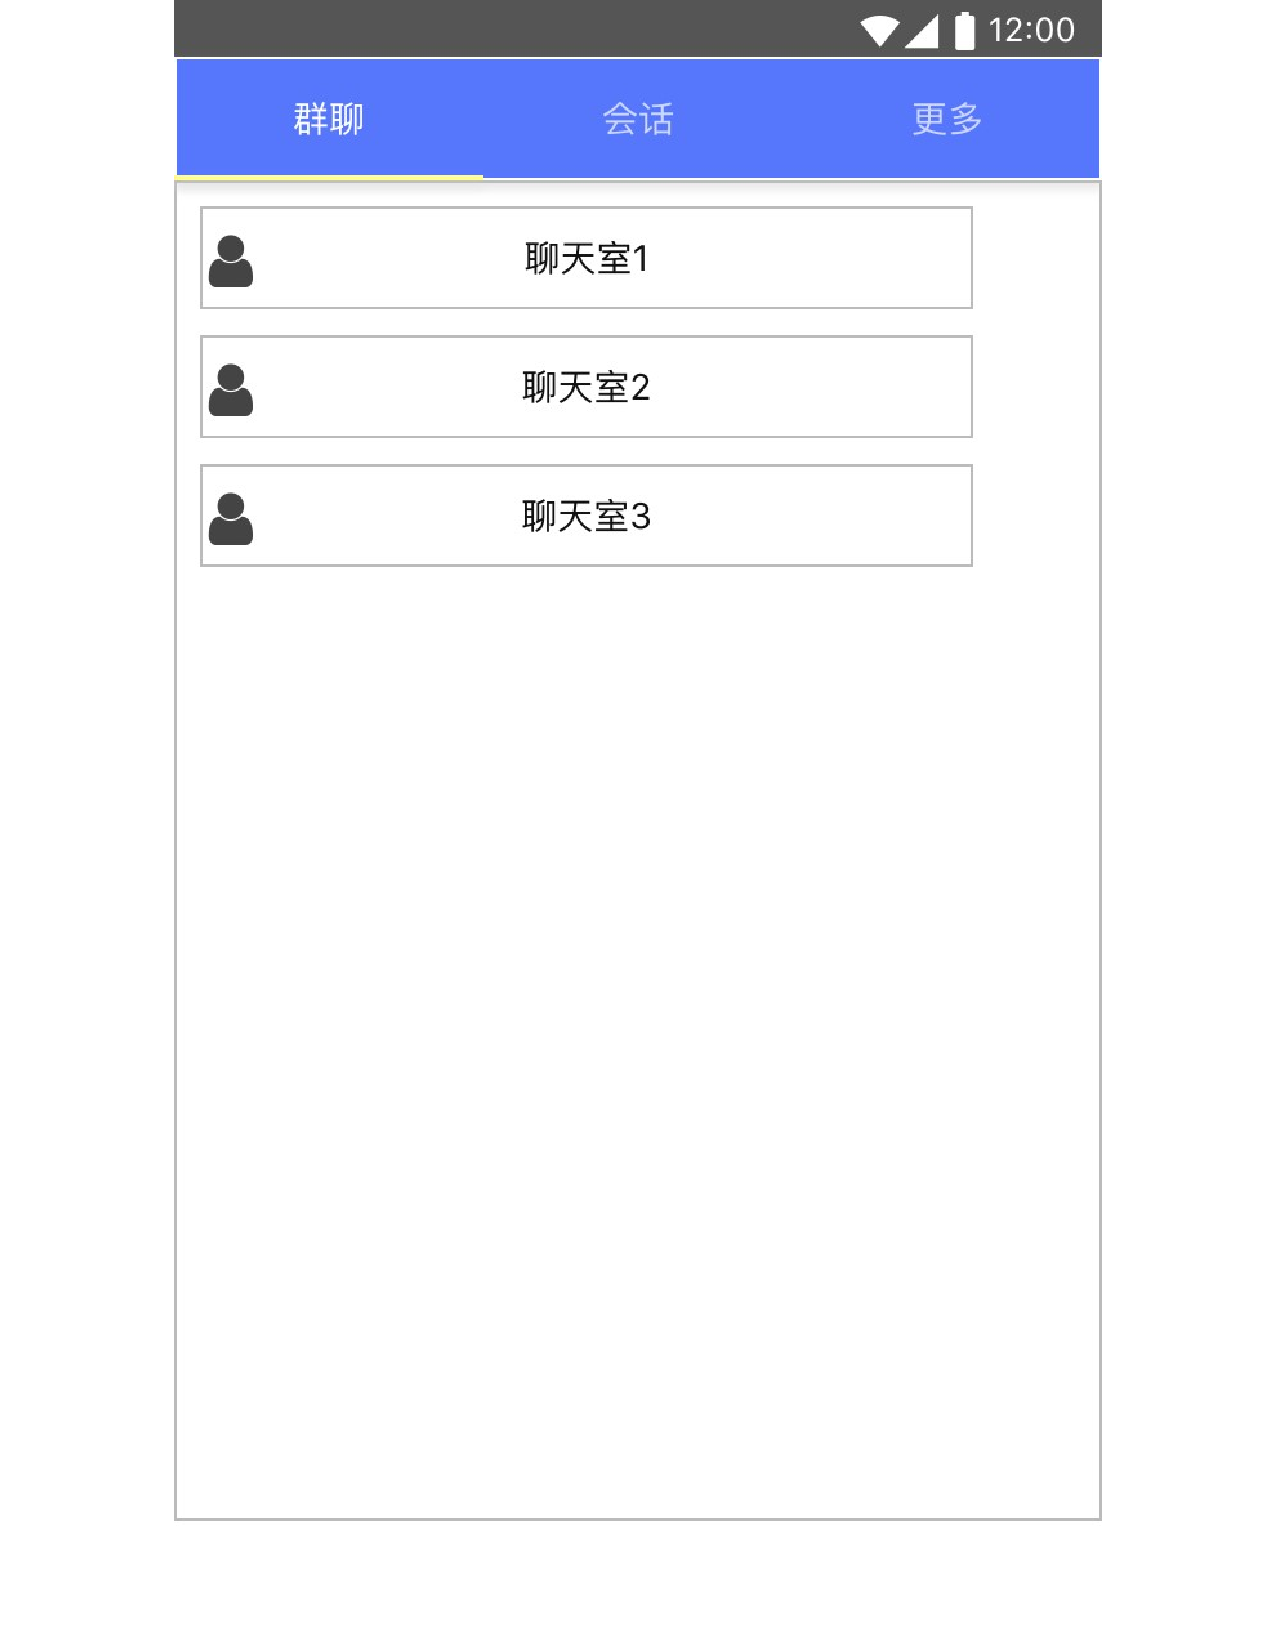
\includegraphics[width=8cm]{Page2_0}
	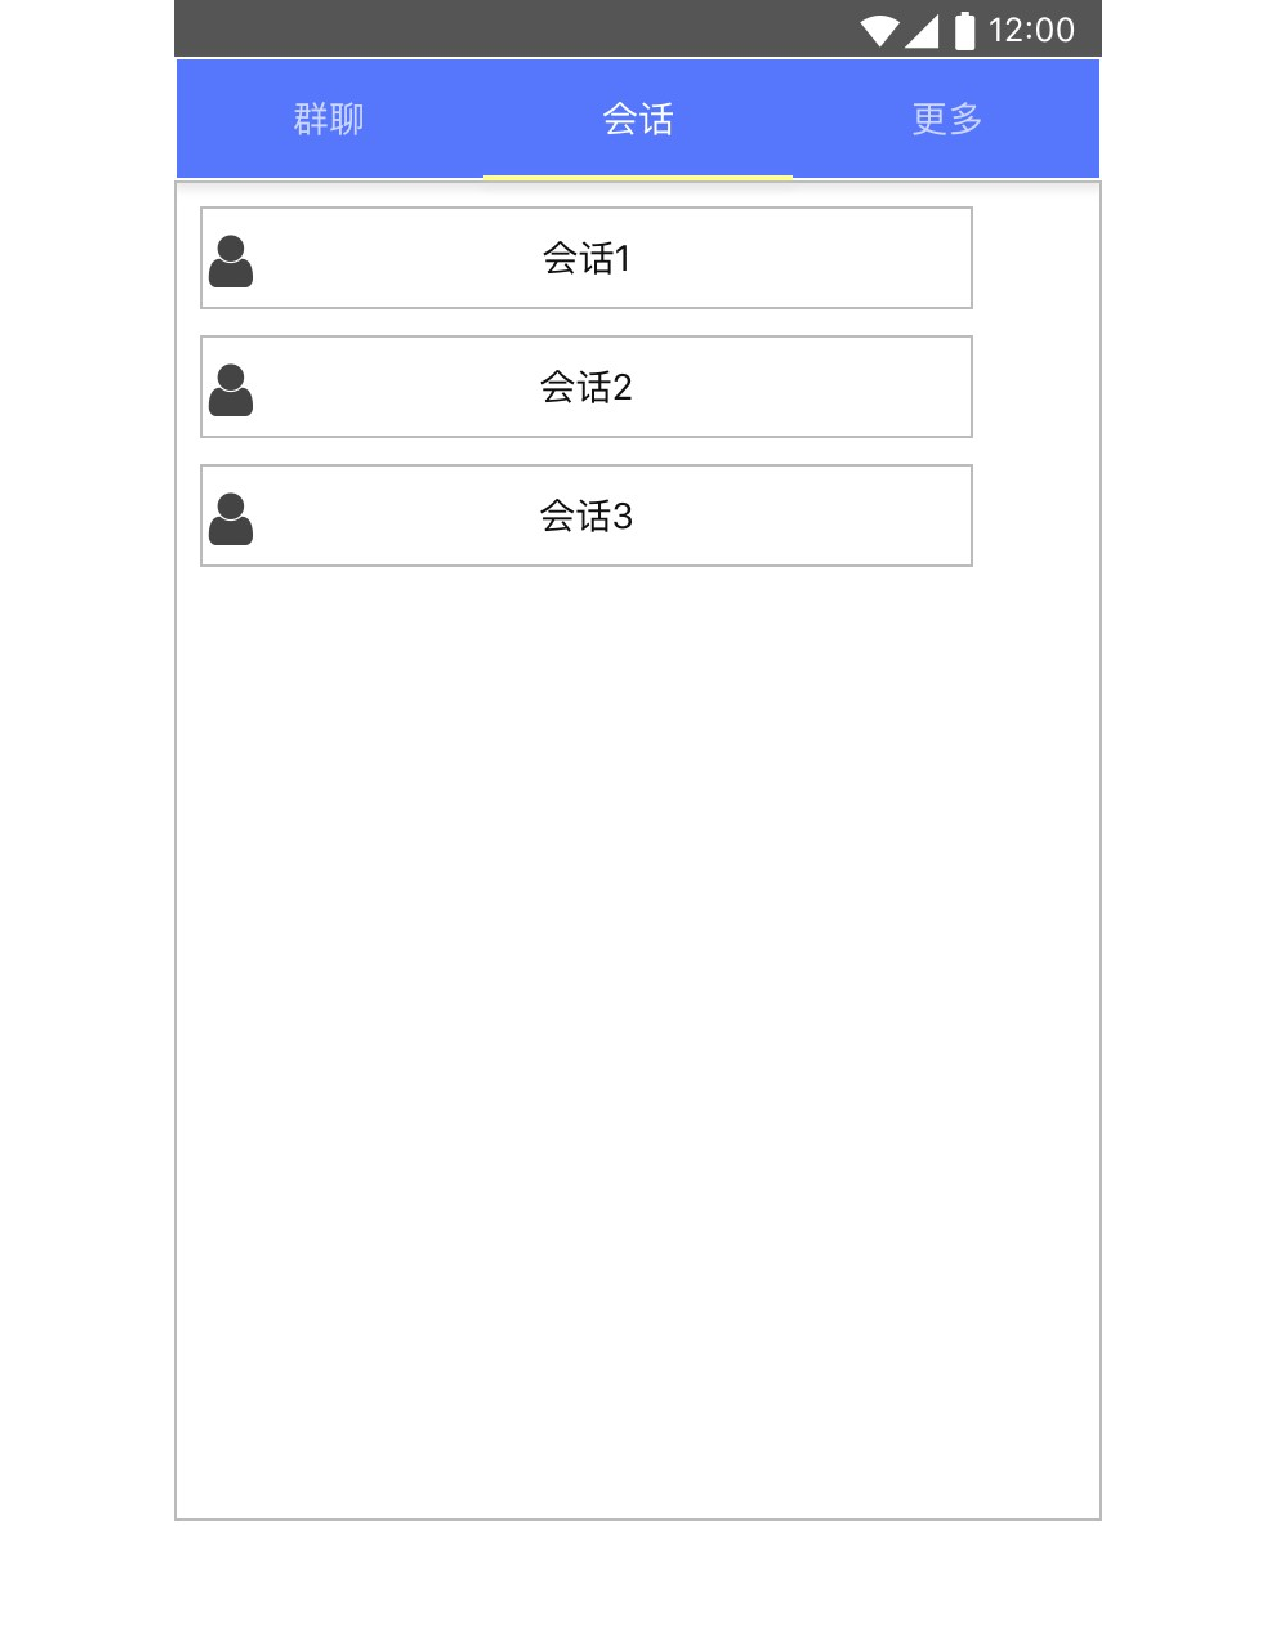
\includegraphics[width=8cm]{Page2_1}
	四张图分别对应 启动页面、登录页面、群聊页面和会画页面
	\label{fig:noted-figure}
   \end{figure}
\subsubsection{启动}
  点击本APP的图标之后,启动项目,首页会显示图片和两个按钮,分别是连接和退出。
\subsubsection{连接}
  点击连接图标之后,如果连接成功,则登录到主界面。
\subsubsection{登录和注册}
  在主界面输入用户名、密码即可登录,如果没有注册,则可以点击“注册”按钮进行注册。一旦注册,则账号和密码被存储到服务器数据库中。
\subsubsection{创建会话}
  登陆之后就可以创建会话、群聊。在上方菜单栏可以选择群聊或会话。通过点击用户列表中的用户就可以发起会话。
\subsubsection{会话界面}
  用户可以在输入框里输入文字并且发送。\\
  用户通过点击最下面的一栏菜单的相应按钮,用户可以发送语音、图片、文件等信息。也可以发起语音通话和视频聊天。
  \begin{figure}[!h]
  	\centering
	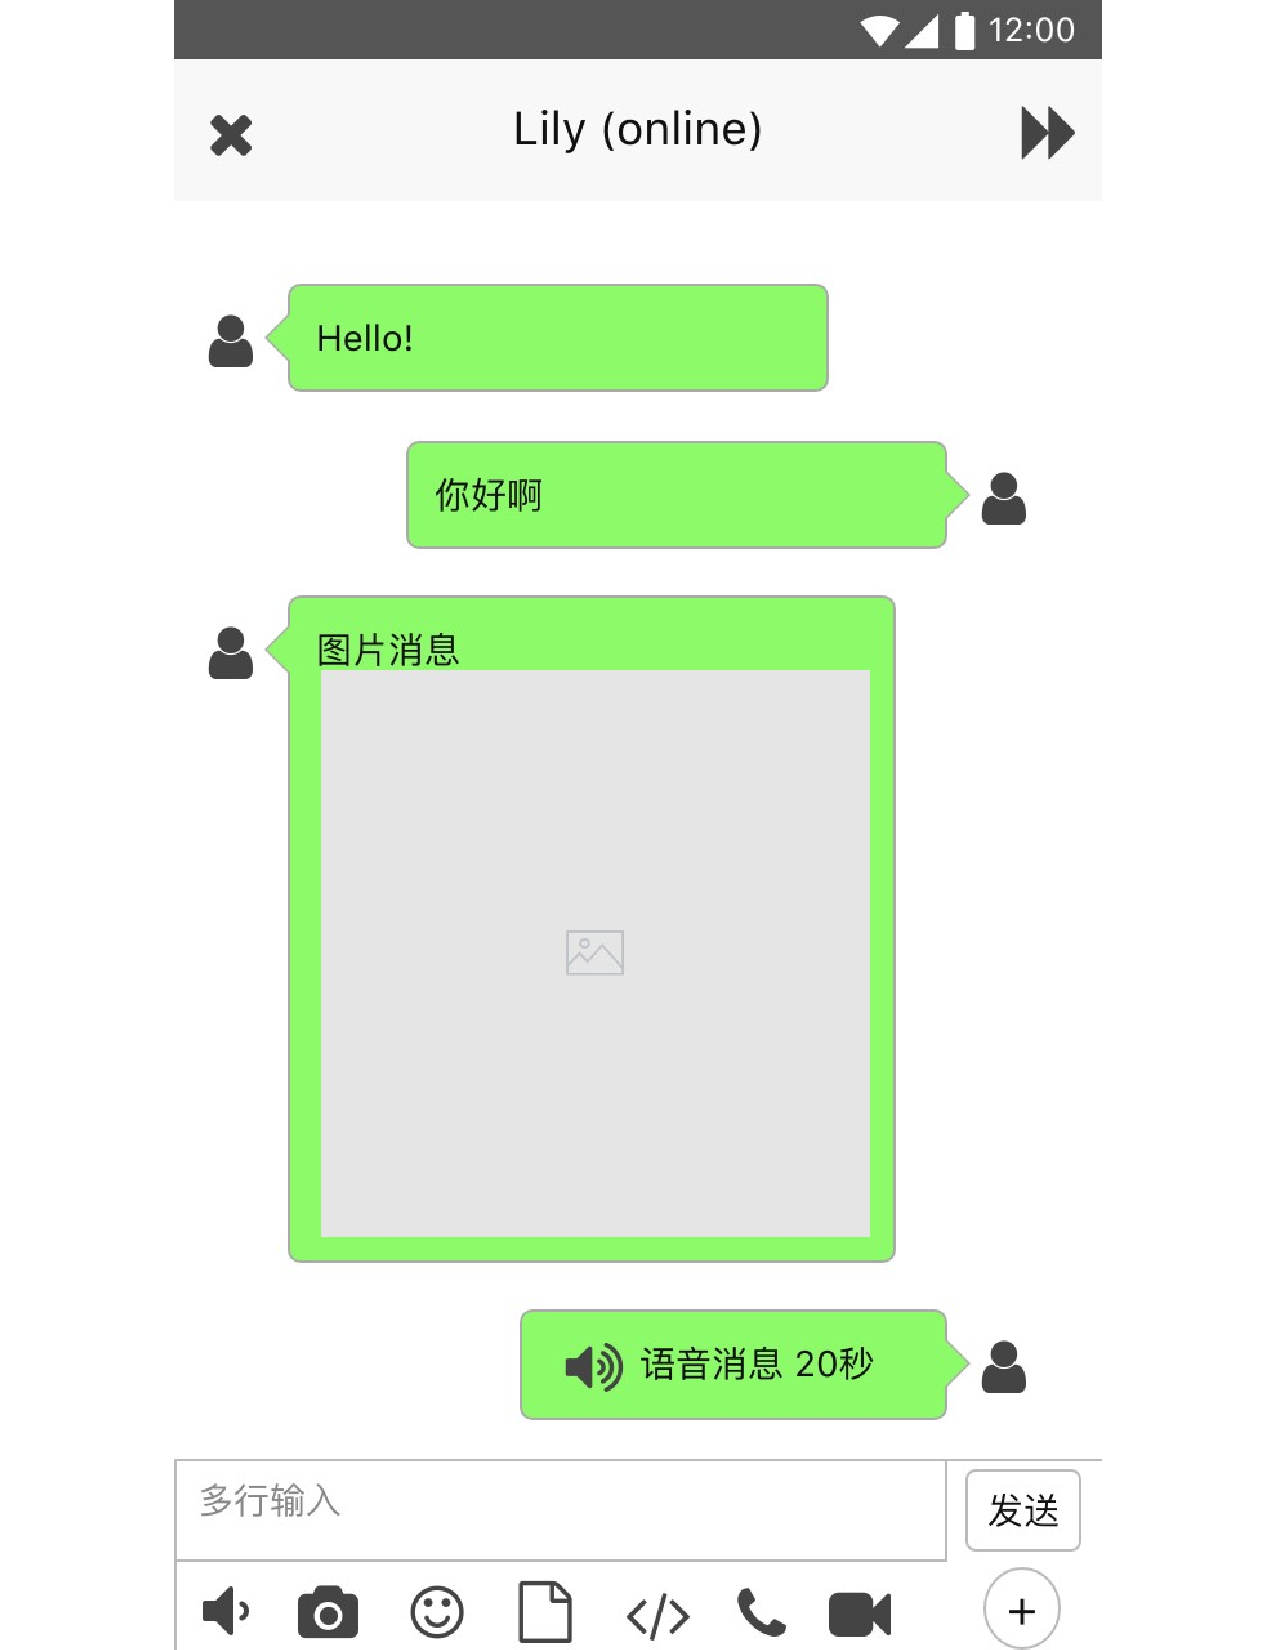
\includegraphics[width=9cm]{Page3}
	\note{聊天界面}
	\label{fig:noted-figure}
  \end{figure}  

\section{性能需求}
\iffalse
<If there are performance requirements, state them here and explain their rationale, to help the developers understand the intent and make suitable design choices. Specifies the timing relationships for real time systems. Such requirements should be made as specific as possible. >

如果有性能方面的需求,在这里列出并解释他们的原理。以帮助开发者理解意图以做出正确的设计选择。在实时系统中的时序关系。保证需求尽可能的详细而精确。

\subsection{性能需求1}
Describes the statically and dynamically quantized requirements on the software (or the interaction between user and the software)
Static quantized requirement could include:
A. Maximum number of terminal supported.
B. Maximum number of users that can use the software at the same time.
C. Maximum number of files and records to be processed
D. Maximum size of  tables and files
Dynamically quantized requirements could include:
A. Specific duration of normal value and peak value of workload (e.g., one hour)
B. Number of event and task and data volume to be processed 
All these requirements should be described by measurable term, for example, saying "95% of the events should be processed in 1 second", instead of saying "the operator need not wait for the business to complete."
Note: The quantized constraint of a detailed requirement should be described in the subsection of the detailed requirement.
本子章节应从整体上描述静态和动态的量化的对软件(或人与软件交互)的需求。

静态的量化需求可能包括:

A. 支持的终端数目。

B. 支持的同时使用的用户数目。

C.处理的文件和记录的数目。

D.表和文件的大小。

动态的量化需求可能包括:

A. 在正常和峰值工作量条件下特定时间段(如一小时)

B. 处理的事务和任务的数目以及数据量。

所有的这些需求应以可测量的术语进行描述,例如所有的操作应在1秒内被处理完成,而不是描述成操作员不必等待操作的完成。

注意: 用于一个具体功能的量化限制通常在该功能的处理子章节中描述。
\fi
\subsection{服务器端性能需求}
\begin{itemize}
	\item 稳定性要求:服务器有效工作时间在99.5\%以上,每次维护时间<24小时。
	\item 业务处理性能要求:能够满足>300个人同时在线,并且满足>50对人能够同时进行较为流畅的视频聊天。据此估算,需要服务器带宽 > 300Mbps。
	\item 数据库性能要求:数据库每秒钟能够进行>400次查询、修改、删除操作,对于每次操作,从收到客户端请求到响应的时间应该小于20ms。
\end{itemize}
\subsection{Android客户端性能需求}
\begin{itemize}
	\item UI界面能够及时响应用户的触摸、点击等事件
	\item 在网络良好的情况下,用户接收、发送消息的延迟<100ms。
	\item 对内存的占用<100MB,不考虑用户文件的情况下,对存储空间的占用<100MB.
	\item 在客户端连续工作的情况下,1小时的耗电量不超过手机基础耗电量的200\%。注:基础耗电量指的是不打开任何外部应用,屏幕开启的情况下手机的耗电量。
	\item 在客户端连续工作的情况下,手机温度相比于未打开客户端的情况没有明显提升。
\end{itemize}
\section{外部接口需求}
\subsection{用户接口}
\iffalse
<The interface of the system with the User and vice versa should be explained in detail. >

详细描述系统与用户之间的接口

This section should include:
A. Features that must be supported by the software for eachman-machine interface. For example, if the user operates from a display terminal, then the following should be included:
		Screen format required
		Page layout and content of report and menu
		Timing sequence for input and output
		Usage of some functional key combinations
B. Every aspect about the use of the system's user interface. It could be a list that shows the user what should do and what should not do.  For example, an option of overlong or overshort message. . And same as other requirements, these requirements should be easily verified. For example, saying "A level 4 typist can finish function X in Z minutes after a one-hour training." instead of "A typist can finish function X"	

这应描述下述内容:

A. 对每种人机界面,软件所必须支持的特性。例如,如果系统用户通过一个显示终端进行操作,那么应包含下述内容:
要求的屏幕格式
页面规划及报告或菜单的内容
输入和输出的相关时序
一些组合功能键的用法

B. 与系统用户接口使用相关的所有方面。这可能只是一个简单的关于系统怎样展示给用户而该做什么和不该做什么的列表。例如提供关于长或短错误消息选项。和所有其它需求一样,这些需求也应能被检验,例如,四级打字员经一小时的培训后能在Z分钟内完成功能X,而不是一个打字员能完成功能X。
\fi
在功能需求里已经详细叙述用户接口。
\begin{itemize}
	\item 需要屏幕分辨率$\ge$800$\times$600, 支持16位以上颜色显示
\end{itemize}
\subsection{软件接口}
\iffalse
<The interface with other system/modules/projects should be explained in detail. >

详细描述与其他系统 /模块 /项目之间的接口

Describes how to use the other (required) software products. (such as data management system, operation system, or algorithm tools package), and the interfaces to other application systems (such as interfaces between the protocol process system and the database management system )
For each required software product, following information should be provided:
A. Name
B. Mnemonic symbol
C. Version number
D. Source
For each interface, this section should:
A. Discuss the objective of the required software.
B. Define the interfaces by content and format of message/function. If the interfaces have been clearly described in other documents, it is not necessary to describe in detail here. But the reference of those documents should be given.

在此应描述如何使用其它(必需的)软件产品(例如,数据管理系统,操作系统,或算法工具包),以及与其它应用系统的接口(例如,协议处理系统和数据库管理系统之间的接口)。

对每个必需的软件产品,应提供下列信息:
A.	名字
B.	助记符
C.	版本号
D.	来源

对每个接口,本部分应:

A .	讨论与本软件产品相关的接口软件的目的。

B.	按消息/函数内容和格式定义接口。如果接口已在其它文档中很清楚地描述,就没有必要在这儿进行详细描述,但需说明应参考的文档。
\fi
\begin{itemize}
\item 客户端
	\begin{itemize}
	\item Windows操作系统(XP以上版本,包含.Net4.0组件)
	\item Android操作系统(5.0.1以上版本)
	\end{itemize}
\item 服务器端
	\begin{itemize}
	\item Ubuntu Server 16.04 操作系统
	\item Mysql数据库
	\item Apache2.0服务器
	\end{itemize}
\end{itemize}




\subsection{硬件接口}
\iffalse
<The interface with other hardware components should be explained in detail. >

详细描述与硬件的接口

Describes the logical features of the interface between the software and hardware components, including the equipment supported and how the equipment and protocol is supported. 

Defines the interfaces according to the content and format of the software/hardware protocol. If the interfaces have been clearly described in other documents, it is not necessary to describe in detail here. But the reference of those documents should be given.

在此描述软件产品和系统硬件组件之间接口的逻辑特征,也包括支持哪些设备、怎样支持这些设备和协议等。
 
按软/硬件协议内容和格式定义接口。如果接口已在其它文档中很清楚地描述,就没有必要在这儿进行详细描述,但需说明应参考的文档。
\fi
\begin{itemize}
	\item 客户端
	\begin{itemize}
		\item 屏幕分辨率$\ge$800$\times$600的手机
		\item 支持麦克风、扬声器或耳机接口
		\item 具有前置摄像头
	\end{itemize}
	\item 服务器端
	\begin{itemize}
		\item 云服务器,含有$\ge$500GB的云硬盘
		\item 具有公共网络接入点
	\end{itemize}
\end{itemize}
\subsection{通讯接口}
\iffalse
<This should specify the various interfaces to communications such as local network protocols, etc.>

详细描述通讯接口,如本地网络协议等。

Defines the interfaces according to the content and format of the message/function. If the interfaces have been clearly described in other documents, it is not necessary to describe in detail here. But the reference of those documents should be given.

按消息/函数内容和格式定义接口。如果接口已在其它文档中很清楚地描述,就没有必要在这儿进行详细描述,但需说明应参考的文档。
\fi
所有信息通过TCP协议发送,要求客户端和服务器支持TCP传输。
\begin{itemize}
	\item 客户端-服务器事件交互信息,采取如下Json字符串格式
    \begin{lstlisting}[language=C++]
   	{
   		"Sender":"sender_id",
   		"SendTime":"send_time",
   		"EventCode":"event_code",
   		"EventParas":
   		{
   			"para1":"para_1",
   			"para2":"para_2"
   		}
   	}
    \end{lstlisting}
    \item 客户端-客户端消息类信息,在头部加上消息发送方、接收方等信息。
    \begin{lstlisting}[language=C++]
    sender_id(32bits)
    receiver_id(32bits)
    datetime(32bits)
    length(32bits)
    payload
    \end{lstlisting}
\end{itemize}
